\documentclass[tikz,border=0pt]{standalone}
\usepackage{tikz}
\usetikzlibrary{arrows.meta, positioning, shapes.geometric, calc, fit, backgrounds}

% --- COLOR DEFINITIONS ---
\definecolor{Garnet}{HTML}{73000A}

% --- STYLES ---
\tikzset{
    % Define a base line width for everything to ensure consistency
    base_width/.style={line width=1pt},
    % Standardized style for all rectangular blocks to ensure identical height
    standard_block/.style={
        rectangle,
        draw=black,
        base_width,
        text width=2.5cm,
        minimum height=1.0cm, % Standardized height for all rectangular blocks
        align=center,
        font=\rmfamily\footnotesize,
        rounded corners=0pt % Strict 90-degree corners
    },
    block/.style={
        standard_block
    },
    % Updated sensor style for cameras to use the Garnet color for the box border
    sensor/.style={
        standard_block,
        draw=Garnet,
        text width=2.2cm
    },
    process/.style={
        standard_block
    },
    decision/.style={
        diamond,
        draw=black,
        base_width,
        aspect=2,
        text width=1.8cm,
        align=center,
        font=\rmfamily\scriptsize
    },
    database/.style={
        cylinder,
        shape border rotate=90,
        draw=black,
        base_width,
        aspect=0.25,
        text width=1.8cm,
        minimum height=1.5cm,
        align=center,
        font=\rmfamily\footnotesize
    },
    arrow/.style={
        ->,
        >={Latex[length=3mm, width=2mm]},
        draw=black,
        base_width
    },
    dashed_arrow/.style={
        ->,
        >={Latex[length=3mm, width=2mm]},
        draw=black,
        dashed,
        base_width
    },
    feedback_arrow/.style={
        ->,
        >={Latex[length=3mm, width=2mm]},
        draw=black,
        dashed,
        base_width
    },
    label_text/.style={
        font=\rmfamily\scriptsize,
        color=black,
        midway,
        auto
    }
}

\begin{document}
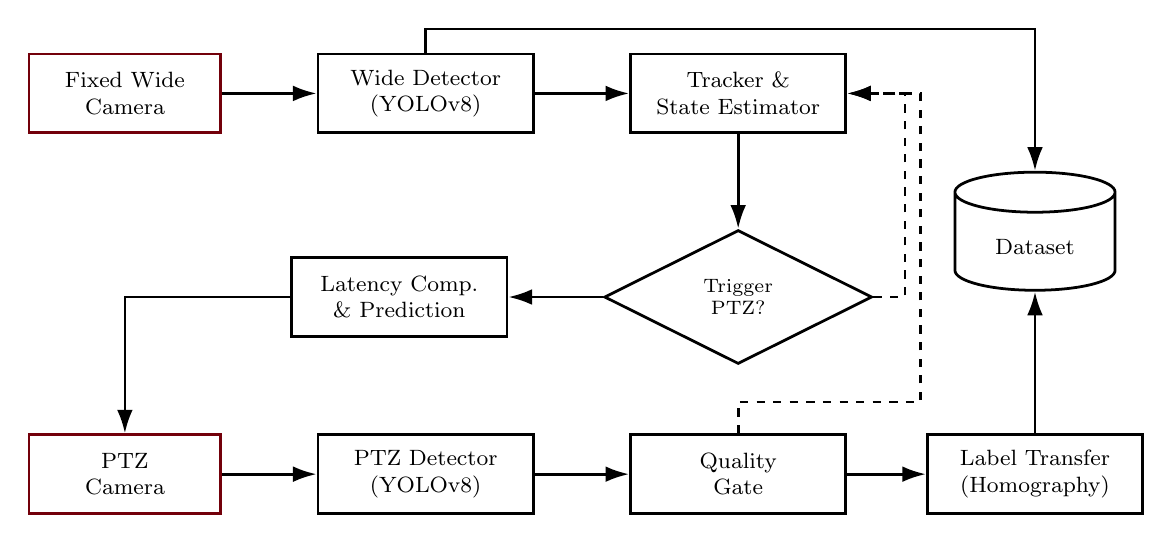
\begin{tikzpicture}[node distance=1.2cm and 1.2cm]

    % --- TOP ROW ---
    \node[sensor] (wide_cam) {Fixed Wide\\Camera};
    \node[block, right=of wide_cam] (wide_det) {Wide Detector\\(YOLOv8)};
    \node[process, right=of wide_det] (tracker) {Tracker \&\\State Estimator};
    
    % --- MIDDLE ROW ---
    \node[decision, below=of tracker] (schedule) {Trigger\\PTZ?};
    \node[process, left=of schedule] (control) {Latency Comp.\\\& Prediction};
    
    % --- BOTTOM ROW ---
    \node[sensor, below=3.8cm of wide_cam] (ptz_cam) {PTZ\\Camera};
    \node[block, right=of ptz_cam] (ptz_det) {PTZ Detector\\(YOLOv8)};
    \node[process, right=of ptz_det] (gate) {Quality\\Gate};
    
    % --- FINAL: DATASET ---
    \node[process, right=1.0cm of gate] (transfer) {Label Transfer\\(Homography)};
    \node[database, above=1.8cm of transfer] (db) {Dataset};

    % --- CONNECTIONS ---
    
    % Wide Loop
    \draw[arrow] (wide_cam) -- (wide_det);
    \draw[arrow] (wide_det) -- (tracker);
    \draw[arrow] (tracker) -- (schedule);
    
    % Decision & Control
    \draw[arrow] (schedule) -- (control);
    \draw[arrow] (control) -| (ptz_cam);
    
    % Continue Path
    \draw[dashed_arrow] (schedule.east) -- +(0.4,0) |- (tracker.east);

    % PTZ Loop
    \draw[arrow] (ptz_cam) -- (ptz_det);
    \draw[arrow] (ptz_det) -- (gate);
    
    % Success Path
    \draw[arrow] (gate) -- (transfer);
    
    % Integration
    \draw[arrow] (transfer) -- (db.south);
    \draw[arrow] (wide_det.north) -- ++(0,0.3) -| (db.north);

    % --- FEEDBACK LOOP ---
    \draw[feedback_arrow] (gate.north) 
        -- ++(0,0.4) 
        -| ($(schedule.east) + (0.6,0)$) coordinate (fb_turn) 
        -- (fb_turn |- tracker.east) 
        -- (tracker.east);

\end{tikzpicture}
\end{document}